\snsubsection{INVERSOR}

\snsubsubsection{Descripción de funcionamiento de un oscilador 555}

RESUMEN

El circuito integrado 555 es un dispositivo de temporización de precisión muy económico, popular y útil, que puede funcionar como un temporizador simple para generar pulsos únicos o retardos largos, o como un oscilador que produce una serie de formas de onda estabilizadas con ciclos de trabajo variables del 50 al 100\%.

El chip temporizador 555 es un dispositivo de 8 pines extremadamente robusto y estable, que puede operar con gran precisión en modo monoestable, biestable o astable. Esto le permite ser utilizado en una amplia variedad de aplicaciones, como temporizadores de un solo disparo o con retardo, generación de pulsos, fuentes de alimentación y convertidores, entre otros. En realidad, puede utilizarse en cualquier circuito que requiera algún tipo de control de tiempo, ya que sus aplicaciones son prácticamente ilimitadas.

El uso más común del temporizador 555 como oscilador es en modo astable, conectando dos resistencias y un capacitor a sus terminales para generar un tren de pulsos con un período de tiempo determinado por la constante de tiempo de la red RC.

FUNCIONAMIENTO

\begin{figure}[H]
    \centering
    \begin{tikzpicture}
        % Paths, nodes and wires:
        \draw (2, 7) to[american resistor, l={$R1$}, label distance=0.02cm] (5, 7);
        \draw (13.25, 4) to[capacitor, l={$C1$}, label distance=0.02cm] (13.25, 1);
        \draw (15.25, 4) to[capacitor, l={$C2$}, label distance=0.02cm] (15.25, 1);
        \draw (5, 6) to[variable american resistor, l={$R2$}, label distance=0.02cm, mirror] (8, 6);
        \draw node[ground] at (9, 1) {};
        \draw (1, 1) -- (1, 8) |- (1.86, 8);
        \draw (5, 7) -- (9.25, 7);
        \draw (4.86, 5) |- (2, 5) -| (2, 7);
        \draw (13.25, 4) -| (13.25, 5) -- (12.25, 5);
        \draw (15.25, 4) -| (15.25, 6) -- (12.25, 6);
        \draw (13.25, 1) -- (1, 1);
        \draw (15.25, 1) -- (13.25, 1);
        \draw (8, 6) -- (9.25, 6);
        \draw (5, 6) -| (5, 7);
        \draw (8.75, 6) -| (8.75, 5.5) -- (8.5, 5.5);
        \draw node[jump crossing] at (2, 8) {};
        \draw (2, 7) -| (2, 7.86);
        \draw (2, 8.14) -- (2, 9.5) -| (14, 8.75) -| (14, 8) -- (12.25, 8);
        \draw node[jump crossing] at (13.25, 3.5) {};
        \draw (13.39, 3.5) -- (15.25, 3.5);
        \draw (13.11, 3.5) |- (5, 3.5) -- (5, 4.86);
        \draw (2.14, 8) -- (9.25, 8);
        \draw node[jump crossing] at (5, 5) {};
        \draw (5.14, 5) -- (9.25, 5);
        \draw (5, 5.14) -| (5, 6);
        \draw (17, 7) to[american voltage source, l={$Vcc$}, label distance=0.02cm] (17, 5);
        \draw (17, 7) |- (14, 9.5);
        \draw (17, 5) |- (15.25, 1);
        \node[shape=rectangle, draw, line width=1pt, inner sep=0, minimum width=2.965cm, minimum height=4.965cm](Rect1) at (10.75, 6.5){} node[anchor=center] at (Rect1.center){$IC555$};
        \node[shape=rectangle, inner sep=0, minimum width=0.465cm, minimum height=0.465cm](Rect2) at (9.5, 8){} node[anchor=center] at (Rect2.center){$1$};
        \node[shape=rectangle, inner sep=0, minimum width=0.465cm, minimum height=0.465cm](Rect3) at (9.5, 7){} node[anchor=center] at (Rect3.center){$2$};
        \node[shape=rectangle, inner sep=0, minimum width=0.465cm, minimum height=0.465cm](Rect4) at (9.5, 6){} node[anchor=center] at (Rect4.center){$3$};
        \node[shape=rectangle, inner sep=0, minimum width=0.465cm, minimum height=0.465cm](Rect5) at (9.5, 5){} node[anchor=center] at (Rect5.center){$4$};
        \node[shape=rectangle, inner sep=0, minimum width=0.465cm, minimum height=0.465cm](Rect6) at (12, 8){} node[anchor=center] at (Rect6.center){$8$};
        \node[shape=rectangle, inner sep=0, minimum width=0.436cm, minimum height=0.465cm](Rect7) at (11.985, 7){} node[anchor=center] at (Rect7.center){$7$};
        \node[shape=rectangle, inner sep=0, minimum width=0.465cm, minimum height=0.465cm](Rect8) at (12, 6){} node[anchor=center] at (Rect8.center){$6$};
        \node[shape=rectangle, inner sep=0, minimum width=0.465cm, minimum height=0.465cm](Rect9) at (12, 5){} node[anchor=center] at (Rect9.center){$5$};
        \path[draw, line width=1pt] (7.5, 5.75) -- (7.25, 5.5) -- (7.5, 5.25) -- (8.5, 5.25) -- (8.5, 5.75) -- (7.5, 5.75) -- cycle  node[anchor=center] at (7.875, 5.5){$555$};
    \end{tikzpicture}
    \caption{Circuito oscilador astable.}
    \label{fig:inversor:IC555}
\end{figure}

El circuito integrado 555 puede conectarse en su modo astable para generar un circuito oscilador muy estable, capaz de producir formas de onda de oscilación libre altamente precisas. La frecuencia de salida puede ajustarse mediante un circuito tanque RC externo compuesto por solo dos resistencias y un capacitor.

El oscilador 555 genera formas de onda cuadradas estabilizadas, ya sea con una frecuencia fija de hasta 500 kHz o con ciclos de trabajo variables entre el 50\% y el 100\%.

En configuración astable requiere que el CI se re-dispare continuamente tras cada ciclo de temporización. Este re-disparo se logra conectando juntos la entrada de disparo (pin 2) y la entrada de umbral (pin 6), permitiendo que el dispositivo funcione como un oscilador astable. Así, un oscilador 555 no tiene estados estables, ya que cambia continuamente de un estado al otro. 

Para que el oscilador produzca un ciclo de trabajo del 50\%, el capacitor de temporización, conectado al pin 6, se tiene que cargar y descargar a través de la resistencia R2 (variable).

Cuando la salida del oscilador 555 está en ALTO, el capacitor se carga a través de R2, y cuando la salida está en BAJO, el capacitor se descarga a través de R2. La resistencia R1 tiene un valor alto y se utiliza para garantizar que el capacitor se cargue completamente hasta alcanzar el mismo valor que la tensión de alimentación.  

El reset (pin 4) debe conectarse a Vcc para evitar que el circuito se desactive involuntariamente, mientras que el control de voltaje (pin 5) se conecta con un capacitor de bajo valor a tierra para mejorar la estabilidad y reducir el ruido. El pin 7 (Descarga) no se usa en esta configuración, ya que la carga y descarga del capacitor ocurren exclusivamente a través de la resistencia R2.
\textcolor{red}{\url{https://www.electronics-tutorials.ws/waveforms/555_oscillator.html}}

\snsubsubsection{Descripción de funcionamiento de un inverosr de medio puente}

RESUMEN

Un inversor es un convertidor que transfiere potencia desde una fuente de continua a una carga de alterna. La función de un inversor es, entonces, cambiar la tensión de entrada de corriente continua en una tensión simétrica de salida en corriente alterna con una magnitud, frecuencia y fase deseada.

Para aplicaciones de baja y mediana potencia, tensiones con formas de onda cuadrada suelen ser suficientes.

En inversores monofásico se utilizan dos topologías básicas: medio puente, el utilizado en este caso, y puente completo. 

FUNCIONAMIENTO

\begin{figure}[H]
    \centering
    \begin{tikzpicture}
        % Paths, nodes and wires:
        \draw (15.5, 8.75) to[curved capacitor, l={$C1$}, label distance=0.02cm] (15.5, 6.75);
        \draw (15.5, 3.75) to[curved capacitor, l={$C2$}, label distance=0.02cm] (15.5, 1.75);
        \draw node[nigfete] (N1) at (11.5, 7.52) {} node[anchor=west] at (N1.text){$Q1$};
        \draw node[nigfete] (N2) at (11.5, 2.77) {} node[anchor=west] at (N2.text){$Q2$};
        \draw (15.5, 6.75) -| (15.5, 3.75);
        \draw (11.5, 6.75) -- (11.5, 3.52);
        \draw (11.5, 8.29) -| (11.5, 8.75) -- (15.5, 8.75);
        \draw (11.5, 2) -| (11.5, 0.25) -- (15.5, 0.25);
        \node[shape=rectangle, draw, line width=1pt, inner sep=0, minimum width=1.215cm, minimum height=0.465cm](Rect1) at (13.375, 5.25){} node[anchor=center] at (Rect1.center){$Carga$};
        \draw (14, 5.25) -- (15.5, 5.25);
        \draw (12.75, 5.25) -- (11.5, 5.25);
        \draw (5, 5.75) to[american voltage source] (5, 4.75);
        \draw (5, 5.75) -| (5, 8.75) -- (7, 8.75);
        \draw (5, 4.75) |- (11.5, 0.25);
        \draw node[npn] at (9.5, 1.73) {};
        \node[shape=rectangle, draw, line width=1pt, inner sep=0, minimum width=1.715cm, minimum height=0.715cm](Rect2) at (7.875, 8.75){} node[anchor=center] at (Rect2.center){$Regulador$};
        \draw (8.75, 8.75) -- (11.5, 8.75);
        \draw node[ground] at (7.875, 8.375) {};
        \draw (15.5, 1.75) -| (15.5, 0.25);
        \draw (10.52, 7.25) to[american resistor, l={$R1$}, label distance=0.02cm] (8.75, 7.25);
        \node[shape=rectangle, draw, line width=1pt, inner sep=0, minimum width=1.215cm, minimum height=0.465cm](Rect3) at (8.125, 7.25){} node[anchor=center] at (Rect3.center){$555$};
        \draw (9.5, 2.5) -| (10.52, 2.5);
        \draw (9.5, 1) -- (9.5, 0.25);
        \draw (8.66, 1.73) to[american resistor, l={$R2$}, label distance=0.2cm] (7.25, 1.75);
        \node[shape=rectangle, draw, line width=1pt, inner sep=0, minimum width=1.215cm, minimum height=0.465cm](Rect4) at (6.375, 1.75){} node[anchor=center] at (Rect4.center){$555$};
        \draw (7, 1.75) -- (7.25, 1.75);
        \draw (9.5, 2.5) to[american resistor, l={$R3$}, label distance=0.02cm] (9.5, 4.5);
        \draw (9.5, 4) -| (9.5, 6) |- (5, 6);
    \end{tikzpicture}
    \caption{Circuito de inversor medio puente.}
    \label{fig:inversor:Medio-Puente}
\end{figure}

En este circuito tenemos dos etapas, una de potencia en la cual encontramos el medio puente conformado por dos transistores mosfet y dos capacitores electrolíticos, y una etapa de control que depende del oscilador 555 visto anteriormente.

Etapa de control

El control del medio puente se realiza a través de la señal de salida del oscilador 555, que se divide en dos ramas. Una de estas ramas se conecta a la gate del transistor Q1 mediante una resistencia, mientras que la otra rama lo hace a la base de un transistor BJT, también a través de una resistencia.

La gate del transistor Q2 se conecta al colector del transistor BJT, que tiene una resistencia conectada a la tensión de alimentación Vcc. El emisor del BJT está conectado a tierra. Este transistor BJT actúa como una compuerta NOT: cuando el oscilador proporciona un impulso alto en la base del BJT, este coloca la gate de Q2 a tierra, evitando que Q2 conduzca. Al mismo tiempo, la gate de Q1 recibe la tensión Vcc, lo que hace que Q1 conduzca.

Cuando la salida del oscilador pasa a un impulso bajo, el comportamiento se invierte. Q1 deja de conducir porque no recibe tensión en su gate. Esto también ocurre en el BJT, que deja de conducir, y la tensión Vcc aplicada a su colector se dirige a la gate de Q2, haciendo que Q2 conduzca.

Así, se logra que solo uno de los dos MOSFETs conduzca en cada ciclo de conmutación, lo que genera la acción complementaria.

Etapa de potencia
Los capacitores electrolíticos conforman un divisor de tensión y estos se mantienen cargados gracias a la tensión entregada por el regulador.

Cuando la salida del oscilador esta en ALTO, como mencionamos, Q1 se activa y Q2 no lo hace. Al activarse Q1 tendremos la tensión que nos otorga el capacitor C1 aplicada en la carga, y el sentido de la corriente es el siguiente:

\begin{figure}[H]
    \centering
    \begin{tikzpicture}
        % Paths, nodes and wires:
        \draw (16, 10) to[curved capacitor] (16, 8);
        \draw (16, 5) to[curved capacitor] (16, 3);
        \draw node[nigfete] at (20, 9) {};
        \draw node[nigfete] at (20, 4.02) {};
        \draw (20, 8.23) -- (20, 4.79);
        \draw (16, 8) -| (16, 5);
        \draw (16, 10) -- (16, 10) -| (20, 9.77);
        \draw (16, 3) -- (16, 3) -| (20, 3.25);
        \node[shape=rectangle, draw, line width=1pt, inner sep=0, minimum width=1.215cm, minimum height=0.465cm](Rect1) at (18, 6.5){} node[anchor=center] at (Rect1.center){$Carga$};
        \draw (18.625, 6.5) -- (20, 6.5);
        \draw (17.375, 6.5) -- (16, 6.5);
        \draw (13, 7) to[american voltage source] (13, 6);
        \draw (13, 7) -| (13, 10) -- (16, 10);
        \draw (13, 6) |- (16, 3);
        \draw (17.5, 7) -- (16.25, 7) -| (16.25, 9.75) -- (19.75, 9.75) -| (19.75, 7) -- (18.5, 7);
        \draw (18.5, 7) -- (18.75, 7.25);
        \draw (18.5, 7) -- (18.75, 6.75);
    \end{tikzpicture}
    \caption{Conmutación 1.}
    \label{fig:inversor:Conmutacion1}
\end{figure}

Cuando el oscilador pasa a estado BAJO, ahora el que se activa es Q2 y ya no lo hace Q1. En este caso la tensión de C2 se aplica en la carga y es negativa ya que la corriente circula en dirección opuesta:

\begin{figure}[H]
    \centering
    \begin{tikzpicture}
        % Paths, nodes and wires:
        \draw (4.25, 7.96) to[curved capacitor] (4.25, 5.96);
        \draw (4.25, 2.96) to[curved capacitor] (4.25, 0.96);
        \draw node[nigfete] at (8.25, 6.96) {};
        \draw node[nigfete] at (8.25, 1.98) {};
        \draw (8.25, 6.19) -- (8.25, 2.75);
        \draw (4.25, 5.96) -| (4.25, 2.96);
        \draw (4.25, 7.96) -- (4.25, 7.96) -| (8.25, 7.73);
        \draw (4.25, 0.96) -- (4.25, 0.96) -| (8.25, 1.21);
        \node[shape=rectangle, draw, line width=1pt, inner sep=0, minimum width=1.215cm, minimum height=0.465cm](Rect1) at (6.25, 4.46){} node[anchor=center] at (Rect1.center){$Carga$};
        \draw (6.875, 4.46) -- (8.25, 4.46);
        \draw (5.625, 4.46) -- (4.25, 4.46);
        \draw (1.25, 4.96) to[american voltage source] (1.25, 3.96);
        \draw (1.25, 4.96) -| (1.25, 7.96) -- (4.25, 7.96);
        \draw (1.25, 3.96) |- (4.25, 0.96);
        \draw (5.75, 3.96) -- (4.5, 3.96) -| (4.5, 1.21) -- (8, 1.21) -| (8, 3.96) -- (6.75, 3.96);
        \draw (5.5, 3.71) -- (5.75, 3.96);
        \draw (5.5, 4.21) -- (5.75, 3.96);
    \end{tikzpicture}
    \caption{Conmutación 2.}
    \label{fig:inversor:Conmutacion2}
\end{figure}

Forma de onda

\begin{figure}[H]
    \centering
    \caption{Forma de onda.}
    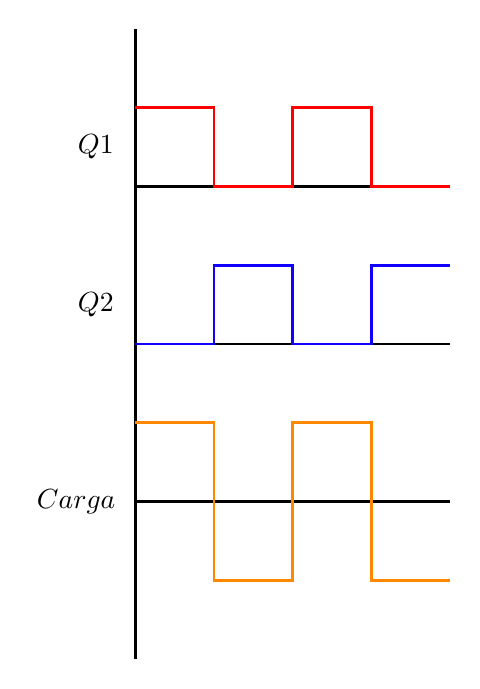
\begin{tikzpicture}
        % Paths, nodes and wires:
        \draw[line width=1pt] (14, 13) -- (14, 5);
        \draw[line width=1pt] (18, 11) -- (14, 11);
        \draw[line width=1pt] (18, 9) -- (14, 9);
        \draw[draw={rgb,255:red,255;green,0;blue,0}, line width=1pt] (14, 12) -- (14, 12) -- (15, 12) -| (15, 11) -- (16, 11) -| (16, 12) -- (17, 12) -| (17, 11) -- (18, 11);
        \draw[draw={rgb,255:red,17;green,0;blue,255}, line width=1pt] (14, 9) -- (15, 9) -| (15, 10) -- (16, 10) -| (16, 9) -- (17, 9) -| (17, 10) -- (18, 10);
        \draw[line width=1pt] (18, 7) -- (14, 7);
        \draw[draw={rgb,255:red,255;green,136;blue,0}, line width=1pt] (14, 8) -- (15, 8) -- (15, 6) -- (16, 6) -| (16, 8) -- (17, 8) -| (17, 6) -- (18, 6);
        \node[shape=rectangle, inner sep=0, minimum width=0.465cm, minimum height=0.465cm](Rect1) at (13.5, 11.5){} node[anchor=center] at (Rect1.center){$Q1$};
        \node[shape=rectangle, inner sep=0, minimum width=0.465cm, minimum height=0.465cm](Rect2) at (13.5, 9.5){} node[anchor=center] at (Rect2.center){$Q2$};
        \node[shape=rectangle, inner sep=0, minimum width=0.465cm, minimum height=0.465cm](Rect3) at (13.25, 7){} node[anchor=center] at (Rect3.center){$Carga$};
    \end{tikzpicture}
    \label{fig:inversor:Forma-onda}
\end{figure}

Las dos primeras formas de onda muestran los pulsos aplicados a los mosfet, donde cada uno recibe el pulso cuando el interruptor complementario está desactivado. El tercer gráfico muestra la forma de onda de voltaje a través de la carga. Esto muestra que la polaridad del voltaje cambia con respecto a la conmutación.

\snsubsubsection{Cálculos}

\section*{Temporizador 555 configurado como oscilador con ciclo de trabajo del 50\%}

Durante cada ciclo, el capacitor se carga hasta el límite superior del comparador \(\left(\frac{2}{3} \times V_\mathrm{DD}\right)\) a través del resistor externo \(R\) y el capacitor \(C\), y luego se descarga hasta el límite inferior del comparador \(\left(\frac{1}{3} \times V_\mathrm{DD}\right)\) a través de los mismos componentes.

La ecuación del voltaje del capacitor en un circuito RC es:
\begin{equation}
V_\mathrm{CAP}(t) = V \left( 1 - e^{-t / RC} \right)
\label{eq:inversor:vcap}
\end{equation}

Reorganizando para obtener el tiempo de carga desde \(\frac{1}{3} \times V_\mathrm{DD}\) hasta \(\frac{2}{3} \times V_\mathrm{DD}\):
\begin{equation}
t_\mathrm{carga} = -RC \times \ln\left(1 - \frac{V_\mathrm{CAP}}{V} \right)
\label{eq:inversor:tcarga_general}
\end{equation}

Si \(V = V_\mathrm{DD}\), \(V_\mathrm{CAP}(t_1) = \frac{1}{3}V_\mathrm{DD}\) y \(V_\mathrm{CAP}(t_2) = \frac{2}{3}V_\mathrm{DD}\), se obtiene:
\begin{equation}
t_\mathrm{carga} = t_2 - t_1 = -RC \times \ln\left( \frac{1}{3} \right) + RC \times \ln\left( \frac{2}{3} \right)
\label{eq:inversor:tcarga_log}
\end{equation}

\begin{equation}
t_\mathrm{carga} = 0{,}693 \times RC
\label{eq:inversor:tcarga_final}
\end{equation}

El tiempo de descarga es igual:
\begin{equation}
t_\mathrm{descarga} = 0{,}693 \times RC
\label{eq:inversor:tdescarga}
\end{equation}

La frecuencia resultante es:
\begin{equation}
f = \frac{1}{t_\mathrm{carga} + t_\mathrm{descarga}} = \frac{1}{2 \times 0{,}693 \times RC}
\label{eq:inversor:frecuencia}
\end{equation}

Para \(C = \SI{0.1}{\micro\farad}\) y \(f = \SI{50}{\hertz}\), la resistencia es:
\begin{equation}
R = \frac{1}{2 \times 0{,}693 \times \SI{50}{\hertz} \times \SI{0.1}{\micro\farad}} = \SI{144.3}{\kilo\ohm}
\label{eq:inversor:resistencia_frecuencia}
\end{equation}

se emplea una resistencia adicional de \SI{10}{\mega\ohm} para asegurar la carga completa del capacitor.

Dentro de las opciones de mosfet a seleccionar, el umbral de conducción \(V_\mathrm{GS(th)} = \SI{2}{\volt} \text{ a } \SI{3}{\volt}\), por lo que VDD tendrá que ser mayor a VCC por \SI{3}{\volt}\, para obtener esta diferencia entre gate y surtidor.

\begin{figure}[H]
    \centering
    \begin{tikzpicture}
        \draw (9.75, 8.46) to[curved capacitor, l={$Vcc/2$}, label distance=0.02cm] (9.75, 6.46);
        \draw (9.75, 3.46) to[curved capacitor, l={$Vcc/2$}, label distance=0.02cm] (9.75, 1.46);
        \draw node[nigfete] (N1) at (5.75, 7.44) {} node[anchor=west] at (N1.text){$Q1$};
        \draw node[nigfete] (N2) at (5.75, 2.48) {} node[anchor=west] at (N2.text){$Q2$};
        \draw (9.75, 6.46) -| (9.75, 3.46);
        \draw (5.75, 6.71) -| (5.75, 3.25);
        \draw (5.75, 8.21) -| (5.75, 8.46) -- (9.75, 8.46);
        \draw (5.75, 1.71) -| (5.75, 1.46) -- (9.75, 1.46);
        \node[draw, rectangle, minimum width=1.215cm, minimum height=0.465cm](Rect1) at (7.75, 4.96){Carga};
        \draw (8.375, 4.96) -- (9.75, 4.96);
        \draw (7.125, 4.96) -- (5.75, 4.96);
        \draw (2.75, 5.46) to[american voltage source, l={$Vcc$}, label distance=0.02cm] (2.75, 4.46);
        \draw (2.75, 5.46) -| (2.75, 8.46) -- (5.75, 8.46);
        \draw (2.75, 4.46) |- (5.75, 1.46);
    \end{tikzpicture}
    \caption{Inversor medio puente con control por 555}
    \label{figure:inversor:calculo-medio-puente}
\end{figure}

\section*{Cálculo de la capacitancia mínima}

\begin{align*}
V_\mathrm{CC} &= \SI{9}{\volt} \\
R_\mathrm{LOAD} &= \SI{100}{\ohm} \\
R_\mathrm{DS(on)} &= \SI{2}{\ohm} \\
T &= \SI{20}{\milli\second}
\end{align*}

\begin{equation}
V_R(t) = \frac{V_\mathrm{CC}}{2} \times e^{-t / RC}
\label{eq:inversor:vrt_descarga}
\end{equation}

\begin{equation}
V_R\left(\frac{T}{2}\right) = \frac{V_\mathrm{CC}}{2} \times \beta
\label{eq:inversor:vr_beta}
\end{equation}

\begin{equation}
\beta = e^{-\frac{T}{2RC}}
\label{eq:inversor:beta}
\end{equation}

\begin{equation}
\ln(\beta) = -\frac{T}{2RC}
\label{eq:inversor:ln_beta}
\end{equation}

\begin{equation}
C \geq \left| \frac{T}{2R \ln(\beta)} \right|
\label{eq:inversor:c_general}
\end{equation}

Con \(\beta = 0{,}9\):
\begin{equation}
C \geq \left| \frac{\SI{20}{\milli\second}}{2 \times \SI{100}{\ohm} \times \ln(0{,}9)} \right| = \SI{950}{\micro\farad}
\label{eq:inversor:c_numerico}
\end{equation}

\section*{Resistencias}

\textbf{Gate del MOSFET:}

\begin{align*}
Q_g &= \SI{70}{\nano\coulomb} \\
t_\mathrm{sw} &= \SI{1}{\micro\second}
\end{align*}

\begin{equation}
I_g = \frac{Q_g}{t_\mathrm{sw}} = \frac{\SI{70}{\nano\coulomb}}{\SI{1}{\micro\second}} = \SI{70}{\milli\ampere}
\label{eq:inversor:ig}
\end{equation}

\begin{equation}
R_g = \frac{V}{I_g} = \frac{\SI{12}{\volt}}{\SI{70}{\milli\ampere}} = \SI{171.4}{\ohm}
\label{eq:inversor:rg}
\end{equation}

\textbf{Resistencia elegida:} \SI{180}{\ohm}, corriente resultante \(> \SI{66}{\milli\ampere}\)

\textbf{Base del BJT:}

\begin{equation}
R_\mathrm{base} = \SI{5.6}{\kilo\ohm} \Rightarrow I_\mathrm{base} = \frac{\SI{12}{\volt}}{\SI{5.6}{\kilo\ohm}} \approx \SI{2.14}{\milli\ampere}
\label{eq:inversor:ibase}
\end{equation}

\textbf{Pull-up:}

\begin{equation}
R = \frac{\SI{12}{\volt}}{\SI{100}{\milli\ampere}} = \SI{120}{\ohm}
\label{eq:inversor:pullup}
\end{equation}

